\section{Algorithme epsilon} \label{sec: annexe_epsilon}
    Soit la série de Gregory pour la fonction $\arctan(x)$
    \begin{align*}
        \arctan(x) = \sum_{n = 0}^\infty(-1)^n\frac{x^{2n + 1}}{2n + 1}
        = x - \frac{x^3}{3} + \frac{x^5}{5} - \frac{x^7}{7} + \dots,
        \label{eq: gregory}
    \end{align*}

    connue pour sa lente convergence. Si l'on pose $x = 1$ dans cette série,
    nous aurions d'un côté $\arctan(1) = \pi$ et de l'autre un série qui
    converge lentement vers cette même valeur. On peut donc se servir, pour
    accélérer la convergence de l'algorithme epsilon définit sur la figure
    \ref{fig: epsilon_tri_array} pour vérifier notre implémentation. Voici un
    graphique qui montre l'erreur commise sur la valeur de $\pi$ de la
    librairie \texttt{numpy} en fonction du nombre de terme dans la série de
    Gregory
    \begin{figure}[h!]
        \centering
        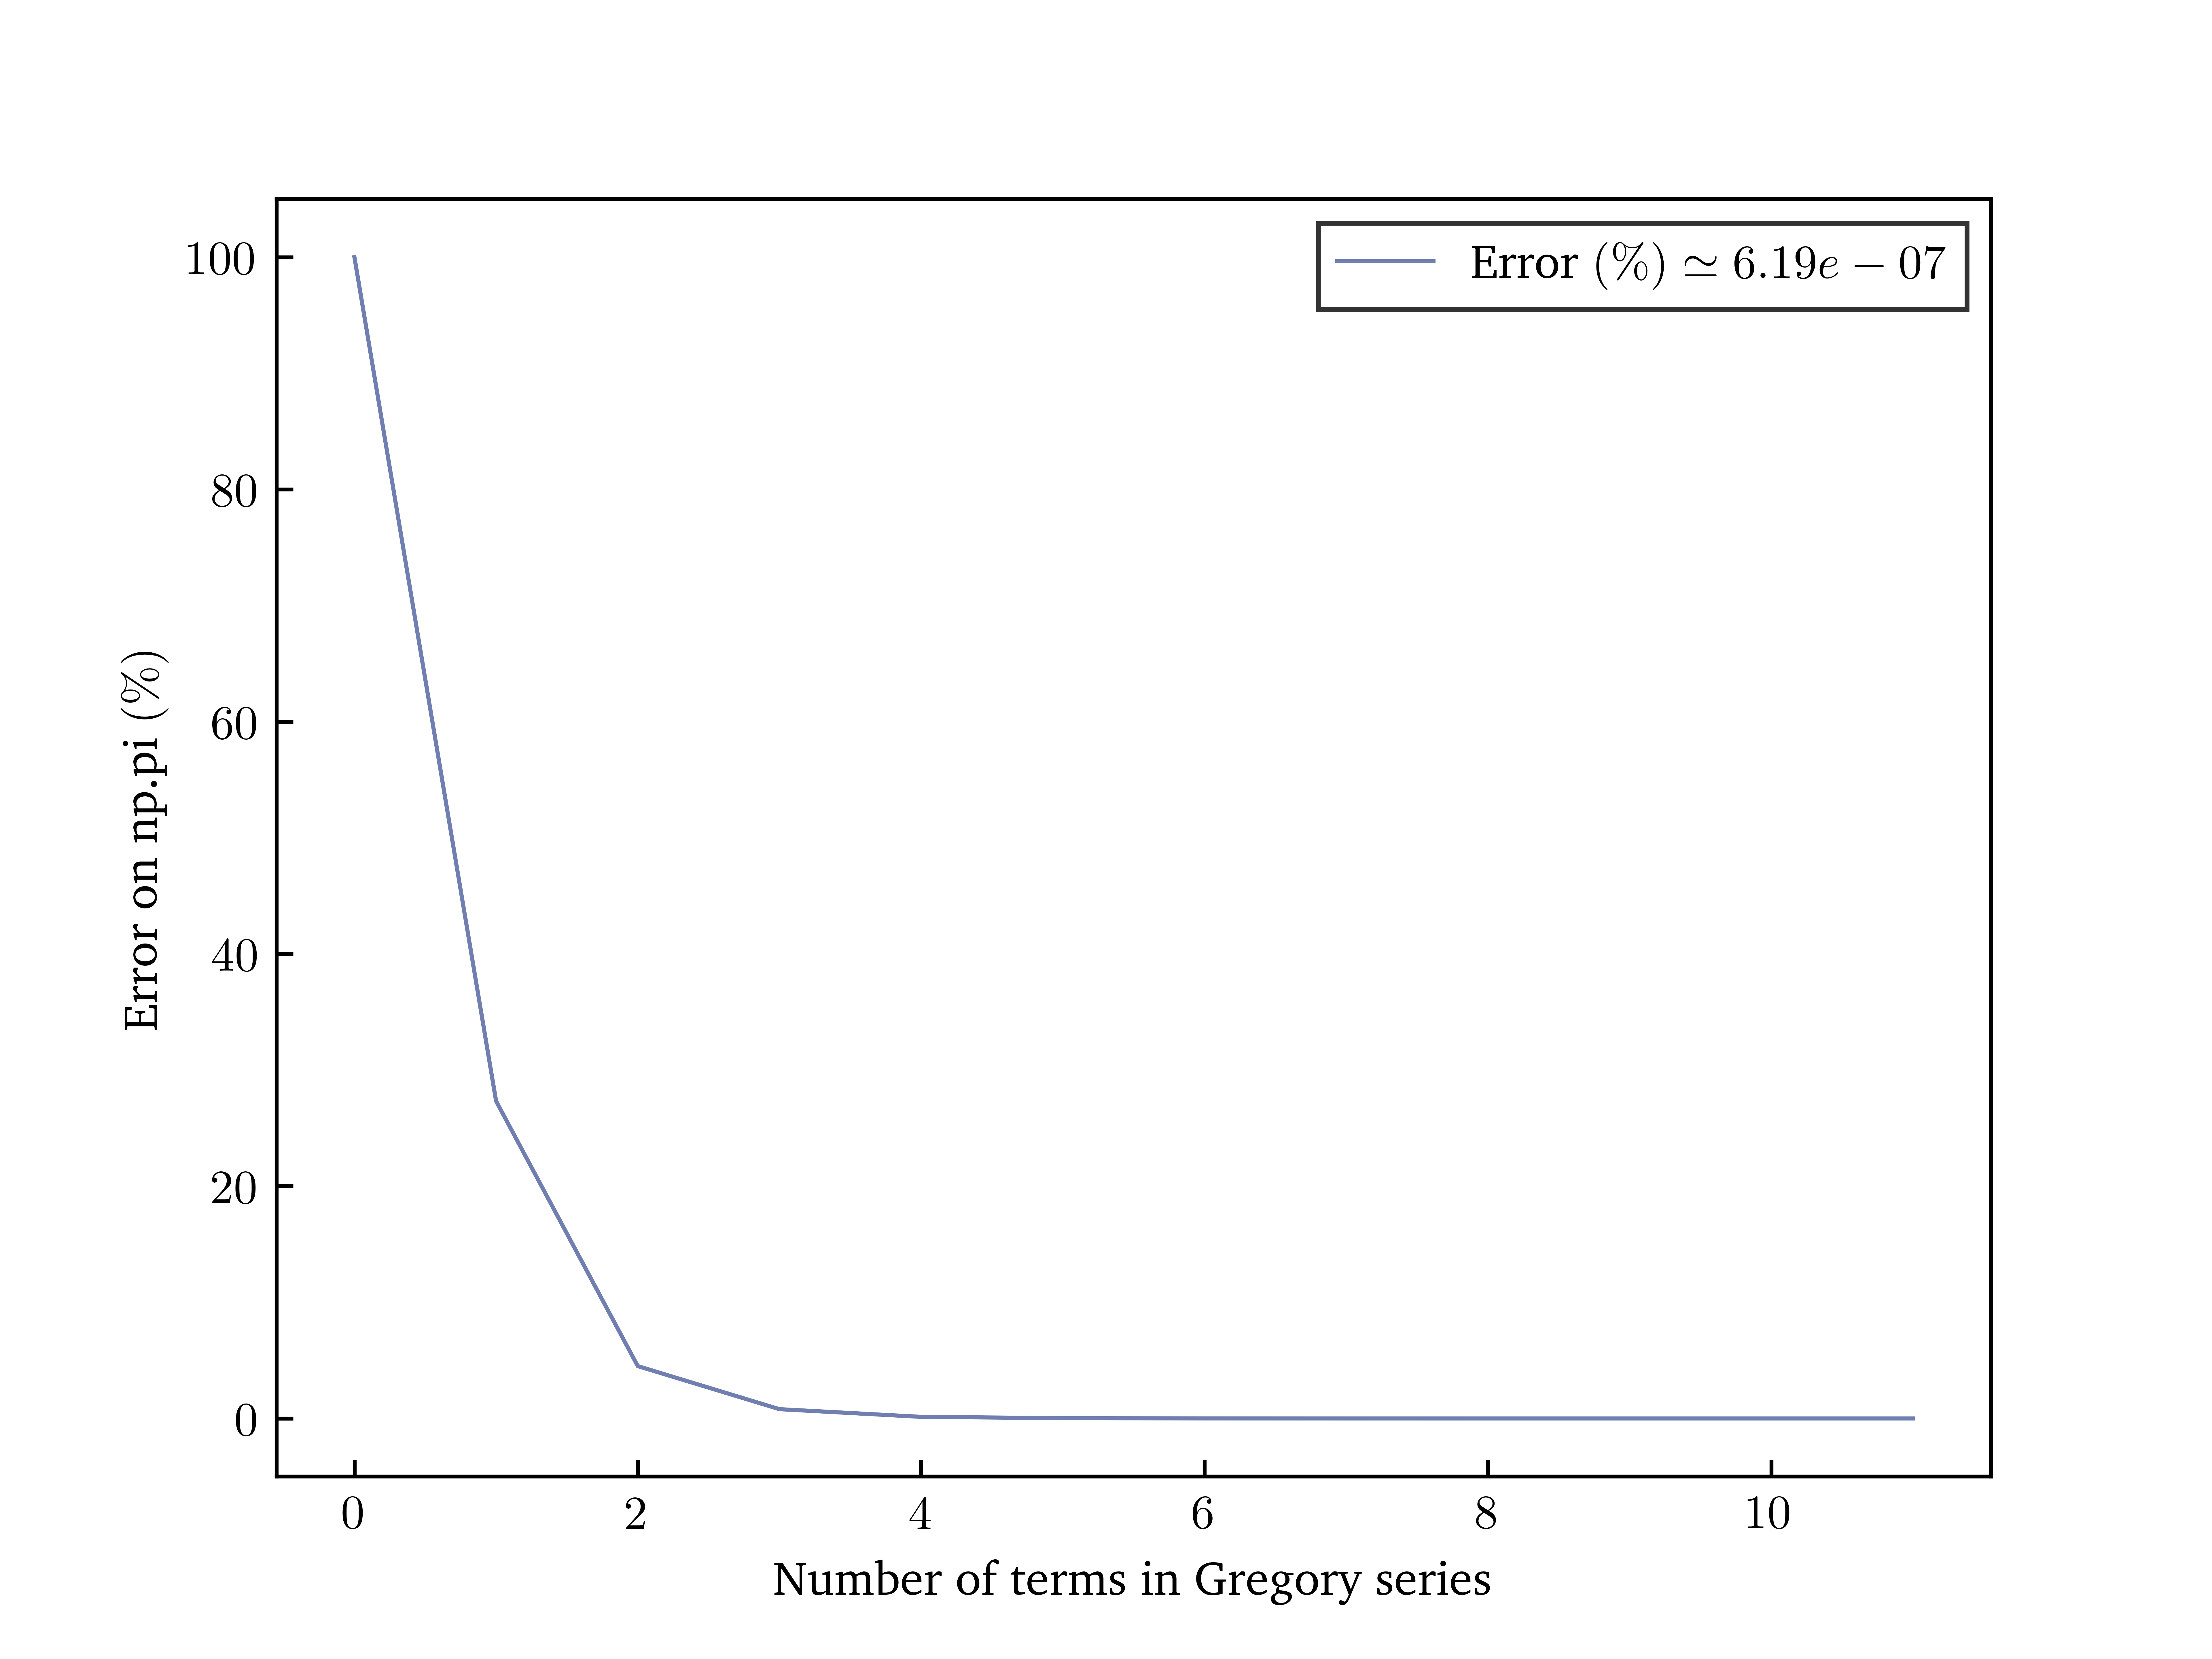
\includegraphics[scale=0.4]{figs/error_percentage.png}
        \caption{Erreur sur l'extrapolation de la série de Gregory (en prenant
        les 12 premiers termes) via l'algorithme epsilon.}
        \label{fig: epsilon_error}
    \end{figure}
    On voit ici sur la figure \ref{fig: epsilon_error} que l'algorithme fait
    effectivement converger la série vers la valeur attendue. On remarque
    qu'avec seulement 5 termes dans la série de Gregory, on peut avoir de très
    bonnes estimations
    \begin{align*}
        \frac{\text{estimation}}{\text{np.pi}}\cdot 100 \simeq
        \frac{3.142342342342342}{3.141592653589793}\cdot 100 \simeq  0.024\%
    \end{align*}
